% This is samplepaper.tex, a sample chapter demonstrating the
% LLNCS macro package for Springer Computer Science proceedings;
% Version 2.20 of 2017/10/04
%
\documentclass[runningheads]{llncs}
%
\usepackage{graphicx}
\usepackage{hyperref}
\usepackage{amsmath}

% Used for displaying a sample figure. If possible, figure files should
% be included in EPS format.
%
% If you use the hyperref package, please uncomment the following line
% to display URLs in blue roman font according to Springer's eBook style:
% \renewcommand\UrlFont{\color{blue}\rmfamily}

%\usepackage[utf8x]{inputenc}
%\usepackage[english,russian]{babel}


\begin{document}
%
\title{Acceleration of Global Search by Implementing Dual Estimates for Lipschitz Constant\thanks{This research was supported by the Russian Science Foundation, project No.\,16-11-10150.}}
%
\titlerunning{Acceleration of Global Search}
% If the paper title is too long for the running head, you can set
% an abbreviated paper title here
%
\author{Roman Strongin\orcidID{0000-0003-0390-6695} 
\and Konstantin Barkalov\orcidID{0000-0001-5273-2471} 
\and Semen Bevzuk\orcidID{0000-0002-3845-5356}
}
%
\authorrunning{R. Strongin et al.}
% First names are abbreviated in the running head.
% If there are more than two authors, 'et al.' is used.
%
\institute{
Lobachevsky State University of Nizhni Novgorod, Nizhni Novgorod, Russia
\email{konstantin.barkalov@itmm.unn.ru}
}
%
\maketitle              % typeset the header of the contribution
%
\begin{abstract}
The paper considers global optimization problems with a black-box objective 
function satisfying the Lipschitz condition. Efficient algorithms for this 
class of problems require reliable estimates of the Lipschitz constant to be 
introduced. Various approaches have been proposed to take into account both
global and local properties of the objective function. In particular, algorithms
using local estimates of the Lipschitz constant have shown their potential.
The new approach presented in this paper is based on simultaneous use of two
estimates: one is substantially larger than the other. 
The larger estimate ensures global convergence and the smaller one reduces 
the total number of trials needed to find the global optimizer.
Results of numerical experiments on the random sample of multidimensional 
functions demonstrate the efficiency of the approach proposed by the authors.  

\keywords{Global optimization \and Multiextremal problems 
\and Lipschitz constant estimates}
\end{abstract}
%
%
%
\section{Introduction}

The paper considers global optimization problems of the form 
\begin{gather}
 \varphi(y^\ast)=\min{\left\{\varphi(y):y\in D\right\}}, \label{problem}\\
 D=\left\{y\in R^N: a_i\leq y_i \leq b_i, \; a_i,b_i\in R, \;  1\leq i \leq N\right\} \label{D},
\end{gather}
where the objective function is a black-box function and it is assumed to satisfy the Lipschitz condition
\[
\left|\varphi(y_1)-\varphi(y_2)\right|\leq L\left\|y_1-y_2\right\|,\; y_1,y_2 \in D,
\]
with the constant $L, \; L<\infty,$ unknown a priori.


The assumption of the objective function to be Lipschitzian is typical of many approaches to the development of the global optimization algorithms \cite{Evtushenko2013,Zilinskas2010,Pinter1996,Strongin2000}. Moreover, the adaptive estimate of the unknown Lipschitz constant, based on the obtained search information, is one of the most important problems being solved in these algorithms. 
The value of the Lipschitz constant affects essentially the convergence rate of the global optimization algorithms. Therefore, the issue of its correct estimate is so important. 
The underestimation of the real value of this constant may result in losing the convergence of the algorithm to the global solution. At the same time, if the value of the constant estimate for the objective function is too large and does not match its real behavior, this will slow down the convergence of the algorithm to the global minimizer. 

Several typical methods of adaptive estimation of the Lipschitz constant are known:
\begin{itemize}
	\item global estimation of the constant $L$ in the whole search domain $D$ \cite{Horst1996,Pinter1996,Strongin2000}.
	\item local estimations of the constants $L_i$ in different subdomains $D_i$ of the search domain $D$ \cite{Kvasov2003,Sergeyev2010,Sergeyev2016}.
	\item the choice of the estimates of the constant $L$ from a set of possible values \cite{Gablonsky2001,Jones1993,Sergeyev2006}.
\end{itemize}

Each of the above approaches has its own advantages and disadvantages. For example, the use of the global estimate over the whole search domain can slow down the convergence of the algorithm to the global minimizer. The use of the local estimates to accelerate the convergence of the method requires an adequate adjustment of the algorithm parameters in order to preserve the global convergence. 

In the present work, we  consider a new algorithm that uses two global estimates of the Lipschitz constant. One of the two estimates is much greater than the other one. 
The larger estimate ensures global convergence and the smaller one reduces the total number of trials needed to find the global optimizer.
The choice of one of the two estimates in the algorithm is performed adaptively during the search phase.

A rigorous substantiation of the proposed approach goes beyond the present initial publication and will be done in the forthcoming works. Here we present the results of numerical experiments that clearly demonstrate the efficiency of the new algorithm. Several hundred multiextremal test problems of various dimensionalities have been solved in the course of numerical experiments.

\section{Global search algorithm and dimensionality reduction}

The adaptation of the efficient algorithms that solve one-dimensional problems to solve multidimensional problems is a typical method to construct global optimization algorithms, see, for example, the diagonal partitions method in \cite{Sergeyev2006} or the simplicial partitions method in \cite{Zilinskas2008}.

In this paper, we follow the approach based on the idea of reducing the dimension with the use of the Peano-Hilbert curves \cite{Sergeyev2013,Strongin2000}, which continuously and unambiguously map the unit interval $[0,1]$ onto the $N$-dimensional cube $D$ from (\ref{D}). By using this kind of mapping, it is possible to reduce the multidimensional problem (\ref{problem}) to a univariate problem
\[
\varphi(y^\ast)=\varphi(y(x^\ast))=\min{\left\{\varphi(y(x)): x\in[0,1]\right\}},
\]
where the function $\varphi(y(x))$ will satisfy a uniform H{\"o}lder condition
\[
\left|\varphi(y(x_1))-\varphi(y(x_2))\right|\leq H\left|x_1-x_2\right|^{1/N}
\]
with the H{\"o}lder constant $H$ linked to the Lipschitz constant $L$ by the relation
$ H=2 L \sqrt{N+3}$ and $y(x)$ is a Peano-Hilbert curve from $[0,1]$ onto $D$.
%Russian
Note that theoretically the Peano-Hilbert curve $y(x)$ is defined as a limit object. Therefore, in practical implementation, only some approximation to the true space-filling curve can be constructed. Some methods for constructing this type of approximations (called evolvents) are considered in \cite{Sergeyev2013,Strongin2000}. In this case, the accuracy of the evolvent approximation to the true curve $y(x)$ depends on the density of the evolvent $m$ (which is a parameter for constructing the evolvent) and is of the order of $2^{-m}$ for each coordinate.

Let us call the process of computing a function value (including the construction of the image $y=y(x)$) as a \textit{trial}, and the pair $\{x, z = \varphi(y(x))\}$ as the outcome of the trial.

The Divide-The-Best global search algorithm used in this paper (according to \cite{Strongin2000}) can be formulated as follows.
The first two trials are executed at 
the points $y^0=y(0), y^1=y(1)$. The choice of the point $y^{k+1},k\geq 1,$  
for the next $(k+1)^{\rm th}$ trial is defined by the following rules.

\begin{enumerate}
	\item 
	Renumber the preimages of all the points $y^i=y(x^i)$
	from the trials already performed  	
%\begin{equation}\label{y_i} 
%y^0=y(x^0), y^1=y(x^1),...,y^k=y(x^k)
%\end{equation}
by subscripts in the increasing order of their coordinates, i.e.
\begin{equation}\label{x_i}
0=x_0<x_1<\dots <x_k=1,
\end{equation}
and associate these with the values $z_i=\varphi(y(x_i)), 0\leq i \leq k,$ 
computed at these points.
\item
Compute the maximum absolute value of the first divided differences
\[
M = \max_{1 \leq i \leq k}\frac{\left|z_i-z_{i-1}\right|}{\Delta_i},
\]
where $\Delta_i=\left(x_i-x_{i-1}\right)^{1/N}$ and let
\begin{equation}\label{mu}
\mu = \left\{
   \begin{array}{lr}
     1, &\textrm{if } M = 0,\\
     M, &\textrm{if } M \neq 0.
   \end{array}
\right.
\end{equation}

\item
For each interval $(x_{i-1}, x_i), \; 1\leq i \leq k,$  calculate the value 
$R(i)$ called the \textit{characteristic} of the interval
\begin{equation}\label{R}
R(i)=\Delta_i+\frac{(z_i-z_{i-1})^2}{r^2\mu^2\Delta_i}-2\frac{z_i+z_{i-1}-2z^*}{r\mu},
\end{equation}
where 
\begin{equation}\label{z}
z^*= \min_{0\leq i\leq k}z_i
\end{equation} 
and the real number $r>1$ is a reliability parameter of the algorithm.
\item 
Select the interval $(x_{t-1},x_t)$ corresponding to the maximum characteristic
\begin{equation}\label{MaxR}
R(t)= \max_{1 \leq i \leq k}R(i).
\end{equation}
\item
Carry out the next trial at the point $x^{k+1}\in(x_{t-1},x_t)$ calculated using
the following formula
\begin{equation}\label{xk1}
x^{k+1} = \frac{x_t+x_{t-1}}{2} - \mathrm{sign}(z_t-z_{t-1})\frac{1}{2r}
\left[\frac{\left|z_t-z_{t-1}\right|}{\mu}\right]^N.
\end{equation}
\end{enumerate}

The algorithm terminates if the condition $\Delta_t < \epsilon$ is satisfied
where $t$ is from (\ref{MaxR}), and $\epsilon>0$ is the predefined accuracy. 

The theory of convergence of this algorithm is provided in \cite{Strongin2000}. 
The algorithm can be efficiently parallelized for shared and distributed memory \cite{Gergel2003}  and for accelerators \cite{Gergel2016}.


\section{Algorithm with Dual Lipschitz Constant Estimates}


The global search algorithm presented in the previous section is intended for solving the multiextremal problems, in which the objective function satisfies the Lipschitz condition. It is not necessary to define the value of the constant for the algorithm convergence. The estimation of the constant is performed in the course of global search based on available search information. 
According to the theorem from \cite{Strongin2000}, the sequence of the trial points $\{y^k\}$ will converge to the global minimizer $y^*$ if the condition 
\begin{equation}\label{cond}
r\mu > 2^{3-1/N}L\sqrt{N+3}
\end{equation}
\noindent is satisfied. Thus,  an appropriate choice of the parameter $r$ from (\ref{R}) allows using the value $(r\mu) / (2^{3-1/N}\sqrt{N+3})$ as an estimate of the Lipschitz constant for the objective function $\varphi(y)$.

Satisfying the condition (\ref{cond}) will be guaranteed if we choose a large enough value of the parameter $r$. However, in this case the method will perform a large number of trials until the stop condition is satisfied.
The choice of a small value of the parameter $r$ (that corresponds to the lower estimate of the Lipschitz constant) would considerably reduce the number of trials but may violate the convergence to the global extremum.

An approach, in which two estimates of the Lipschitz constant are used in the rules of the algorithm, seems quite promising. 
This approach implies the use in the algorithm of two parameters $r_{glob}$ and $r_{loc}$, where $r_{glob} > r_{loc}>1$.


%Russian
The rules of the algorithm with two estimates of the Lipschitz constant reproduce the ones of the global search algorithm completely except Rule 3 (the computation of the characteristic) and Rule 4 (search for the interval with the maximum characteristic).

The new rule for calculating the characteristic $R(i)$ of the interval $(x_{i-1}, x_i)$ will consist of the following operations:
\begin{itemize}
\item
Calculate the value $R_{glob}(i)$ corresponding to the larger estimate of the Lipschitz constant
\[
R_{glob}(i)=\Delta_i+\frac{(z_i-z_{i-1})^2}{r_{glob}^2\mu^2\Delta_i}-2\frac{z_i+z_{i-1}-2z^*}{r_{glob}\mu}.
\]
\item
Calculate the value $R_{loc}(i)$ corresponding to the smaller estimate of the Lipschitz constant
\[
R_{loc}(i)=\Delta_i+\frac{(z_i-z_{i-1})^2}{r_{loc}^2\mu^2\Delta_i}-2\frac{z_i+z_{i-1}-2z^*}{r_{loc}\mu}.
\]
\item
Determine the characteristic $R(i)$ as
\begin{equation}\label{pho}
R(i) = \max\{\rho R_{loc}(i),R_{glob}(i)\}, \textrm{where} \; \rho = \left(\frac{1-1/r_{glob}}{1-1/r_{loc}}\right)^2,
\end{equation}   
\end{itemize}

%Russian
The new rules for finding the interval with the maximum characteristic will be as follows:
\begin{itemize}
\item 
Select the interval $(x_{t-1},x_t)$ corresponding to the maximum characteristic $R(t)= \max_{1 \leq i \leq k}R(i)$.
\item
Fix the value $r = r_{loc}$ if $\rho R_{loc}(t) > R_{glob}(t)$, otherwise fix $r=r_{glob}$.
\item
Use this value of $r$ in Rule 5 of the algorithm in the computing of the next trial point.
\end{itemize}


This method for computing the characteristic can be substantiated as follows. 
%Russian
Each search iteration will yield an interval with the current minimum value $z^*$ from (\ref{z}) at one of its boundaries. In the final phase of the search, this interval will correspond to the interval containing the global minimum, i.e. it will be the best one in terms of conducting further trials within it.

Let the current minimum value of $z^*$ from (\ref{z}) be achieved at the left point of the $i^{\rm th}$ interval, i.e. $z^* = z_{i-1}$. 
As proven in \cite{Strongin2000}, according to the rule (\ref{R}) the following inequality will be true: 
\[
R(i) \geq \Delta_i \left( 1 - 1/r \right)^2.
\]
Therefore, for the estimates of the characteristics $R_{loc}(i)$ and $R_{glob}(i)$ calculated with different parameters $r_{loc}$ and $r_{glob}$, the following relation will hold:
\[
	\Delta_i \left( 1 - 1/r_{glob} \right)^2 > \Delta_i \left( 1 - 1/r_{loc} \right)^2.
\]

Thus, when choosing the largest of the characteristics in accordance with
\[
R(i) = \max\{R_{loc}(i),R_{glob}(i)\}
\]
%as a rule,
the characteristic $R_{glob}(i)$ corresponding to the higher estimate of the Lipschitz constant will be chosen; the lower estimate (which speeds up the process of refining the current solution) will not be used.
However, if we multiply the lower estimate for the characteristic $R_{loc}(i)$ by the coefficient $\rho$ in accordance with (\ref{pho}), then such lower estimates will be equal, 
thus the choice of the characteristic $R_{loc}(i)$ corresponding to the lower estimate of the Lipschitz constant will become more likely.

%Consequently, two lower estimates of the two characteristics of current best interval $R_{loc}(i)$ and $R_{glob}(i)$ calculated with different parameters $r_{loc}$ and $r_{glob}$ will take different values. However, if the former is multiplied by the coefficient $\rho$ from (\ref{pho}), the lower estimates of the characteristics of the best interval would match each other that would make the characteristics calculated for other intervals comparable as well.

\section{Numerical Experiments}

%Russian
A numerical comparison of the algorithms was carried out by solving several series of problems generated by the GKLS generator \cite{Gaviano2003}. This generator of multiextremal functions is widely used to compare global optimization methods (see, for example, \cite{Barkalov2018,Sergeyev2006,Sergeyev2015}). In this study, six series each containing 100 problems of dimensions $N = 3,4,5$ were solved. For each dimension, \textit{Simple} and \textit{Hard} problems were generated, differing in the size of the attraction regions for local extremums and global extremum.
The problem was considered solved if the method conducted the trial at a point that was in the $\delta$-neighborhood of the global minimizer $y^\ast$, 
i.e. $\left\|y^k-y^\ast\right\| <\delta\left\|b-a\right\|$, where  $a$ and $b$ are the boundaries of the search domain $D$.

%The numerical comparison of the algorithms has been carried out using the GKLS test problem generator \cite{Gaviano2003}. This generator of multiextremal functions is often used for the investigations of the global optimization algorithms ~\cite{Barkalov2018,Paulavicius2014,Sergeyev2015}. Six GKLS classes of 100 differentiable test functions of the dimensions $N = 3,4,5$ have been used. For each dimension, both \textit{Hard} and \textit{Simple} classes have been considered. The difficulty of a class was increased either by decreasing the radius of the attraction region of the global minimizer, or by decreasing the distance from the global minimizer $y^\ast$ to the domain boundaries. The global minimizer $y^\ast$ was considered to be found, if the algorithm generated a trial point $y^k$ in the vicinity of the global minimum, i.e. $\left\|y^k-y^\ast\right\| <\delta\left\|b-a\right\|$, $a$ and $b$ are the boundaries of the search domain $D$. 


Each series of problems has been solved by the original global search algorithm (GSA) and by the method with two estimates of the Lipschitz constant (GSA-DL). The evolvent constructed using the parameter $m = 10$ was used for the dimensionality reduction in both algorithms. The relative accuracy of the solution search was $\delta = 0.01$. 
The maximum allowable number of iterations per problem was $K_{max} = 10^6$.

The averaged numbers of iterations performed by the algorithms are presented in Table \ref{tab:1}.
For the GSA method the values of the parameter $r=4.8$ when solving the problems of the \textit{Simple} class and $r=5.6$ when solving the problems of the \textit{Hard} class were used. 
These values are the minimum ones (with the accuracy 0.1), at which all problems have been solved successfully.
When solving the problems from the above classes by the GSA-DL method, the value of the parameter $r$ specified above was selected for the upper estimate of the Lipschitz constant, i.e. the value $r_{glob} = r$ was set, which was complemented by the values $r_{loc}=1.8$, $r_{loc}=2.1$ and $r_{loc}=2.4$. 
The number of unsolved problems is specified in brackets.

\begin{table}
	\caption{Average number of iterations}
	\label{tab:1}
	\center
	\begin{tabular}{ccccccccc}
		\hline\noalign{\smallskip}
		 & \multicolumn{2}{c}{$N=3$} & & \multicolumn{2}{c}{$N=4$} & & \multicolumn{2}{c}{$N=5$}  \\
		\noalign{\smallskip} \cline{2-3} \cline{5-6} \cline{8-9} \noalign{\smallskip}
		 & \textit{Simple} & \textit{Hard} & & \textit{Simple} & \textit{Hard} & & \textit{Simple} & \textit{Hard}  \\
		\noalign{\smallskip} \hline \noalign{\smallskip}
									AGS	&	2444	&	5345	& &	28415	&	77470	& & 25220(1) & 126138(4)		\\
AGS-DL, $r_{loc}=1.8$	&	1372	&	2632	& &	13273	&	37715	& &	12702    & 94296(1)			\\
AGS-DL, $r_{loc}=2.1$	&	1502	&	2805	& &	14826	&	38843	& &	15213    & 90792(2)			\\
AGS-DL, $r_{loc}=2.4$	&	1567	&	2868	& &	19447	&	40342	& &	18239    & 106438(2)		\\
		\noalign{\smallskip}\hline
	\end{tabular}
\end{table}

\begin{figure}
\begin{minipage}{0.47\linewidth}
\center{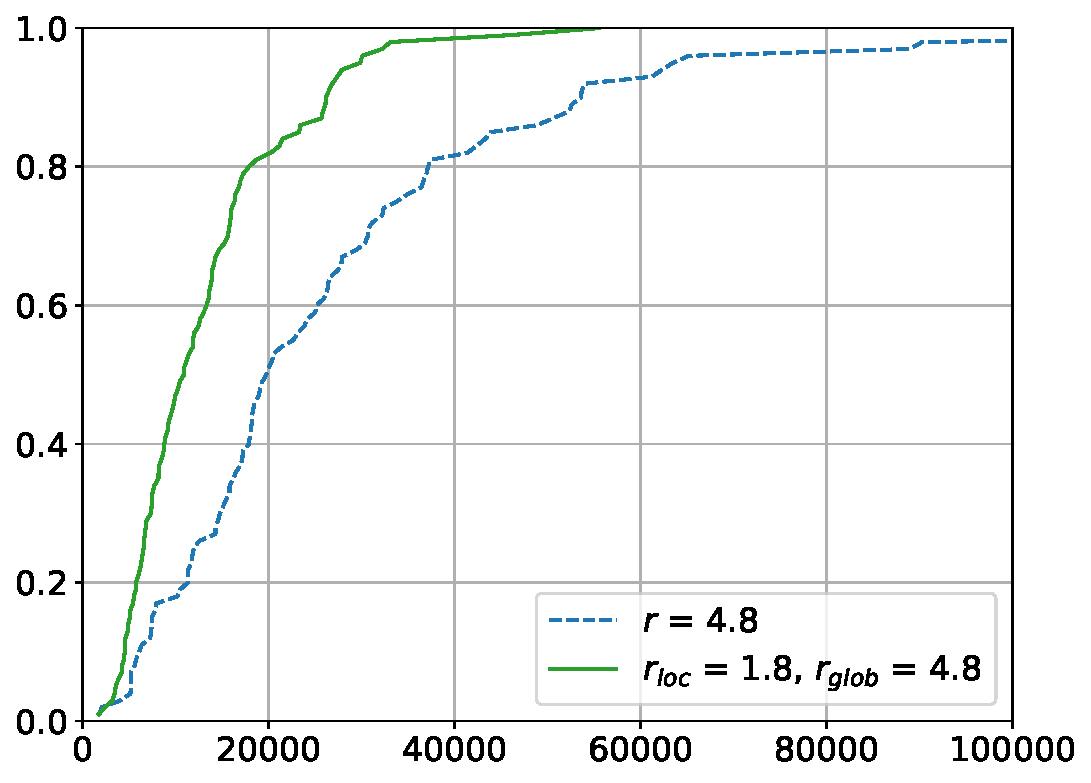
\includegraphics[width=1.0\linewidth]{Operating_characteristic_gklss_4.pdf} {\scriptsize \\ (a)}}
\end{minipage}
\hfill
\begin{minipage}{0.47\linewidth}
\center{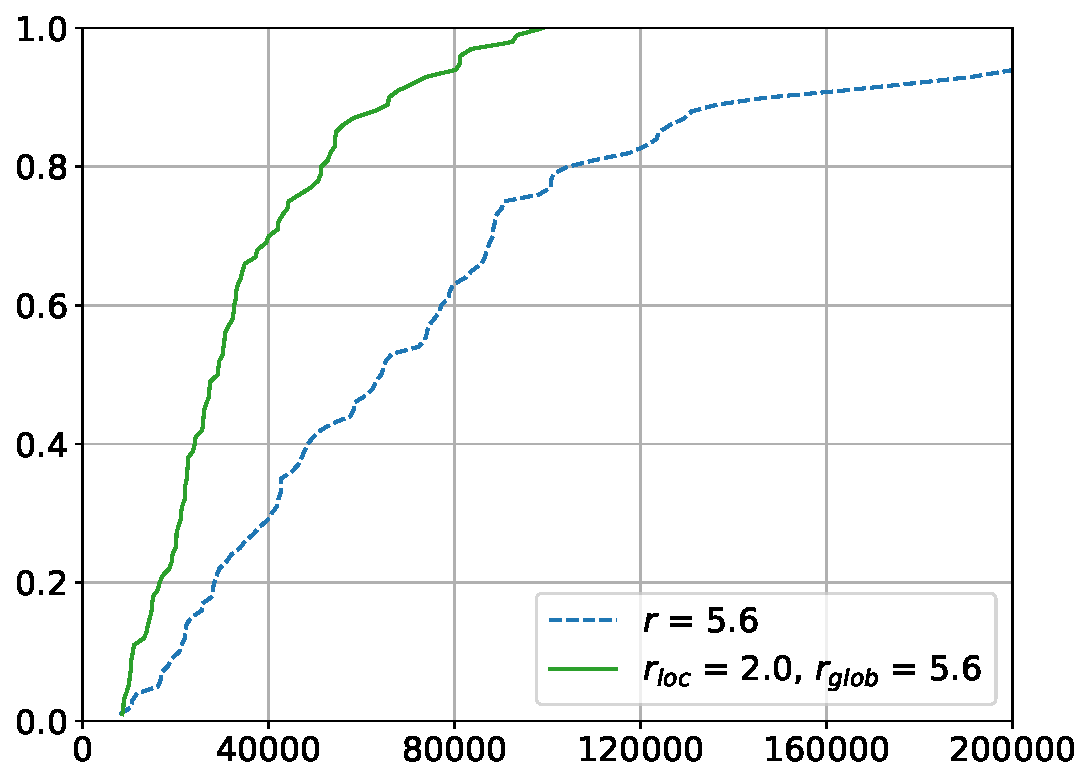
\includegraphics[width=1.0\linewidth]{Operating_characteristic_gklsh_4.pdf} {\scriptsize \\ (b)}}
\end{minipage}
\caption{Operational characteristics for GKLS \textit{Simple} (a) and \textit{Hard} (b) classes, $N=4$.}
\label{oper4}
\end{figure}


The advantages of the GSA-DL algorithm over its prototype are also confirmed by the operational characteristics of the algorithms as well. Assume a series of test problems to be solved. The results of solving the series can be presented by a function $p(k)$ featuring the fraction of the total number of problems solved in $k$ iterations. Such a function will be called the \textit{operational characteristic} of the algorithm. 

The operational characteristics for the GSA and GSA-DL methods obtained when solving the \textit{Simple} and \textit{Hard} problem series with the dimensionalities $N=4$ and $N=5$ are presented in Fig. \ref{oper4} and Fig. \ref{oper5}, respectively. The values of the parameters $r$ used for estimating the Lipschitz constant are given in the figures.

\begin{figure}
\begin{minipage}{0.47\linewidth}
\center{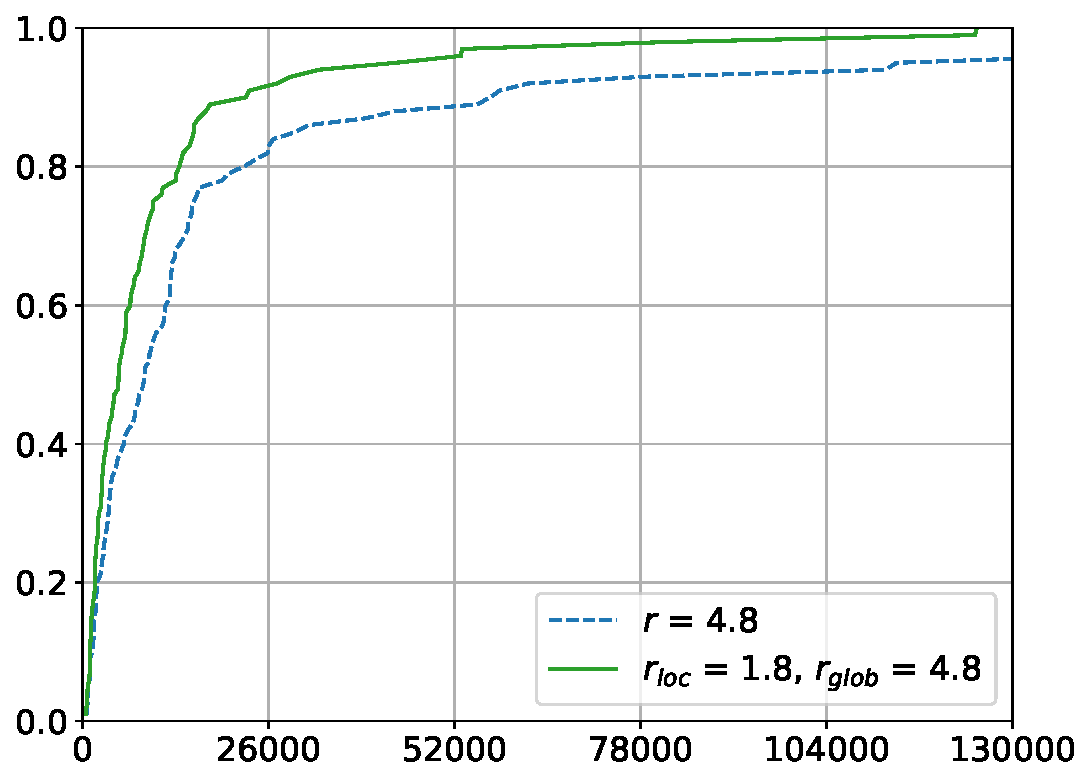
\includegraphics[width=1.0\linewidth]{Operating_characteristic_gklss_5.pdf} {\scriptsize \\ (a)}}
\end{minipage}
\hfill
\begin{minipage}{0.47\linewidth}
\center{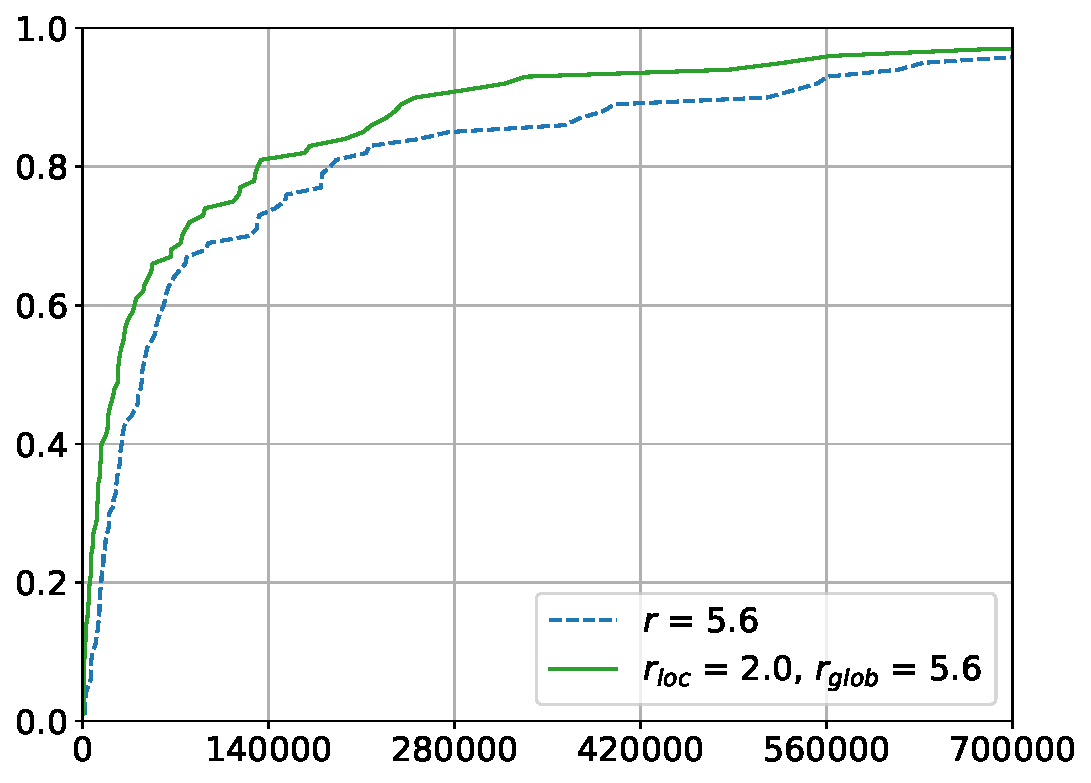
\includegraphics[width=1.0\linewidth]{Operating_characteristic_gklsh_5.pdf} {\scriptsize \\ (b)}}
\end{minipage}
\caption{Operational characteristics for GKLS \textit{Simple} (a) and \textit{Hard} (b) classes, $N=5$.}
\label{oper5}
\end{figure}


The lower curves in Fig. \ref{oper4} and Fig. \ref{oper5} feature the characteristics of the GSA method whereas the upper ones, those of the GSA-DL. Such relative positions of the curves show the algorithm with two estimates of the Lipschitz constant is much faster on average when solving the problem series than the algorithm using a single estimate of the constant.
%Russian
Note that to solve problems of all classes (except for the \textit{Hard} class at $N=5$) the GSA-DL method requires about half as many trials as the GSA. The deterioration of the results in the case of the \textit{Hard} class at $N=5$ is explained by the complexity of this class' functions, which have a large attraction region of local minima and a narrow attraction region of the global minimum. To correctly solve such problems, the GSA-DL method often uses a higher estimate of the Lipschitz constant, thus reducing the speed difference of the GSA and GSA-DL algorithms.

% ---- Bibliography ----
%
% BibTeX users should specify bibliography style 'splncs04'.
% References will then be sorted and formatted in the correct style.

\bibliographystyle{splncs04}
\bibliography{bibliography}

%\begin{thebibliography}{8}
%\end{thebibliography}
\end{document}
